% Chapter 2

\chapter{Background} % Write in your own chapter title
\label{Chapter2}
\lhead{Chapter 2. \emph{Background}} % Write in your own chapter title to set the page header

This work makes heavy use of different techniques  and tools mostly 
in the context of compiler construction. To simplify the rest of the thesis 
this chapter explains them as far as necessary, thus we may take
them for granted afterwards. As most of the key ideas will suffice, 
some details will be omitted. 
Interested readers have to fall back on the further readings instead. 


\section{LLVM - The LLVM Compiler Infrastructure}
\label{LLVM}
The Low Level Virtual Machine is a compiler infrastructure designed to optimize
during compile time, link time and runtime. Originally designed for C and C++, 
many other frontends for a variety of languages exist by now. The source is 
translated into an intermediate representation (LLVM-IR), which is available 
in three different, but equivalent forms. There is the in-memory compiler IR, 
the on-disk bitcode representation and human readable assembly language.
The LLVM-IR is a type-safe, static single assignment based language,
designed for low-level operations. It is capable of 
representing high-level structures in a flexible way.
Due to the fact that LLVM is built in a modular 
way and can be extended easily, most of the state of the art analysis and
optimization techniques are implemented and shipped with LLVM. Plenty of other
extensions, e.g., Polly, can be added by hand. 


\subsection*{Further Reading}

\begin{itemize}
  \item A Compilation Framework for Lifelong Program Analysis \& Transformation
    \cite{LLVM:CGO04}  
  \item \url{http://www.llvm.org} \nocite{LLVM:Online}
\end{itemize}


\clearpage
\section{The Polyhedral Model}
The polyhedral model is a mathematical way to describe the iteration space of 
loop nests, or more specifically a very restricted subset of them.
It became popular as it abstracts from the given source and applies loop
optimizations in a pure mathematical way. Formulating optimization problems 
in terms of linear equations yields an optimal solution with regard to a given
property, e.g., data-locality or parallelism.

%\begin{definition}[Polyhedron] ~\\
  %A polyhedron P in an $n$-dimensional space restricted by $m$ inequalities is defined as:
  %\[ \text{P}:= \{ x \in \mathbb{Z}^n \, |\, Ax\leq b \text{ where $A\in\mathbb{Z}^{m*n} $ and $ b\in\mathbb{Z}^{m}$ are constant } \} \]
  %\label{def:polyhedron}
%\end{definition}



%\lstset{frame=none}
%\begin{wrapfigure}[]{l}{0.4\textwidth}
  %\vspace*{-5mm}
  %\subfloat[Example loop nest]{%
    %\begin{minipage}[c][0.6\width]{%
           %0.35\textwidth}
           %\centering%
      %\lstinputlisting{Primitives/Code/Polytope2d.c}
      %\label{lst:Polytope2dC}
    %\end{minipage}
  %} 
  
  %\subfloat[Iteration space for listing \ref{lst:Polytope2dC}]{%
    %\begin{minipage}[c][1.2\width]{%
           %0.35\textwidth}
           %\centering%
      %\includegraphics[width=0.9\textwidth]{Figures/Polytope2d.eps}
      %\label{lst:Polytope2dPolyhedral}
    %\end{minipage}
  %}


  %\caption{The polytope model in action }
  %\label{fig:Polyhedron2d}
%\end{wrapfigure}
%\resetlst
Within the polyhedral model the iteration space is represented as a $\mathbb{Z}$-polyhedron,
simply spoken a geometric object with flat surfaces existing in a space of any
dimensionality. To do so, it is necessary that the iteration space 
can be described as solution set of affine inequalities
(equation \ref{eq:IterationSpace}), where the loop bounds are encoded in a translation
($b$) and the steppings in a matrix ($A$). 
\begin{equation}
  \text{Iteration Space IS } := \{ x \in \mathbb{Z}^n \, |\, Ax\leq b \text{ with $A\in\mathbb{Z}^{m*n} $, $ b\in\mathbb{Z}^{m}$  } \} \label{eq:IterationSpace}
\end{equation}
%Definition \ref{def:polyhedron} restrict all (integer) points within the polyhedron
%to be solutions of an affine system of inequalities which can be derived from
%the source code. The example in figure \ref{fig:Polytope2d} shows how these 
%inequalities (figure \ref{lst:Polytope2dInequalities}) 
%are derived from the source presented in listing \ref{lst:Polytope2dC} and how 
%the resulting polyhedral (figure \ref{lst:Polytope2dPolyhedral}) looks like.
%[TODO unify the two examples]

%For clarification it is worth to say
%that some authors e.g., Benabderrahmane et al. \cite{BPCB10} use the term 
%polyhedron instead of polytope. 
%As each loop corresponds to a dimension of the vector space the
%dimension of the polyhedron is determined by the depth of the loop nest. 
In addition to the points of the iteration space, the polyhedral model is also
capable of representing loop carried dependencies between two iterations. 
Figure \ref{fig:ExampleLoopNest} illustrates this by relating a simple loop 
nest({\footnotesize A}) to its representation in the polyhedral 
model({\footnotesize B}). 
Note that we do not distinguish between the base pointers 
(here \texttt{A} and \texttt{B}) when we draw dependencies. 
This is feasible because we have to respect all dependencies in order to perform 
loop transformations. 

%The main benefit of 
%this representation is that transformations can be done in an optimal manner
%using an integer linear programming solver which maximizes the loop nest for 
%e.g., parallelism.
An optimization within the model (which is in fact a composed
affine transformation) could yield 
%with the additional advantage that they implicitly apply 
%traditional loop optimizations including tiling, skewing, loop interchange and
%unrolling. 
%Using the example in listing \ref{lst:ExampleLoopNest} again we may end up with
a loop nest as presented in listing \ref{lst:ExampleLoopNestTransformed}. 
Data-locality has been increased by introducing the two inner most loops which
also remove the data dependency from the outer most one, 
thus the whole loope nest may be executed in parallel now.

\lstset{frame=none}
\begin{figure}[htbp]
  \centering
  \subfloat[Simple loop nest]{%
    \begin{minipage}[c][0.6\width]{%
           0.45\textwidth}
           \centering%
    \lstinputlisting{Primitives/Code/ExampleLoopNest.c}
    \label{lst:ExampleLoopNest}
    \end{minipage}
  } 
  \subfloat[Polyhedral representation for listing \ref{lst:ExampleLoopNest}]{%
    \begin{minipage}[c][0.6\width]{%
           0.45\textwidth}
           \centering%
    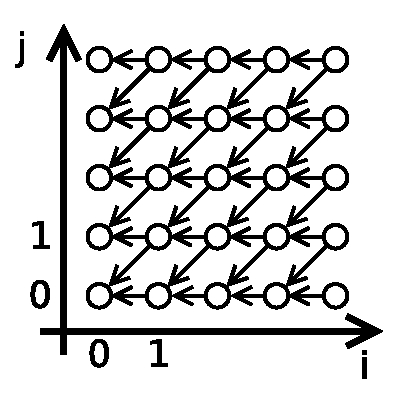
\includegraphics[width=0.55\textwidth]{Figures/ExampleLoopNestPolytope2.eps}
    \label{fig:ExampleLoopNestPolytope}
    \end{minipage}
  }
  \caption{An example loop nest with its polyhedral representation}
  \label{fig:ExampleLoopNest}
\end{figure}
\resetlst

\lstset{frame=none}
\begin{figure}[htbp]
  \centering
\begin{tabular}{c}
    \lstinputlisting{Primitives/Code/ExampleLoopNestTransformed.c}
  \end{tabular}
  \caption{Optimized version of listing \ref{lst:ExampleLoopNest}}
  \label{lst:ExampleLoopNestTransformed} 
\end{figure}
\resetlst



\lstset{frame=none}
\begin{figure}[htbp]
  \centering
\end{figure}
\resetlst

\subsection*{Further Reading}
\begin{itemize}
  \item The Polyhedral Model is More Widely Applicable Than Yoy Think \cite{BPCB10}
  \item Loop Parallelization in the Polytope Model \cite{Lengauer93loopparallelization}  
  \item A practical automatic polyhedral parallelizer and locality optimizer \cite{Bondhugula:2008:PAP:1379022.1375595}
  \item PoCC - The Polyhedral Compiler Collection \cite{PoCC:Online}
  \item Polyhedral parallelization of binary code \cite{Pradelle:2012:PPB:2086696.2086718}
  \item Putting Polyhedral Loop Transformations to Work \cite{BCGST03} 
\end{itemize}

\clearpage

\section{Polly - A Polyhedral Optimizer For LLVM}
\label{Polly}
Exploiting parallelism and data-locality in order to balance the workload
and to improve cache locality are the main goals of the Polly research project.
The polyhedral model is used as abstract mathematical representation to get optimal
results for a particular objective. The three-step approach of Polly first detects
maximal loop nests suitable for polyhedral representation. These representations
are analyzed and transformed before they are converted to code (here LLVM-IR)
again. In the case of Polly the code generation is capable of generating thread 
level parallelism and vector instructions. The code regions Polly is interested 
in, are called static control parts, or short SCoPs. Such a SCoP is 
the most central entity within Polly and crucial for any kind of argumentation.
%Apart from the
%following descriptions figure \ref{fig:PollyArchitecture} provides an overview
%of the architecture of Polly.

\begin{definition}[Affine Transformation] ~\\
  Affine transformations are linear transformations followed by a translation,
  thus they can be written as:
  \[ f(x_1,\dots,x_n) := A_1\, x_1 + \dots + A_n\, x_n + b\]

  \label{def:AffineTransformation}
\end{definition}

\begin{definition}[Canonical Induction Variable] ~\\
  An induction variable is canonical if it starts at zero and steps by one.
  \label{def:CanonicalInductionVariable}
\end{definition}

\subsection{Static Control Parts}
%\begin{wrapfigure}[]{r}{0.15\textwidth}
  %\centering
  %%\vspace*{-5mm}
  %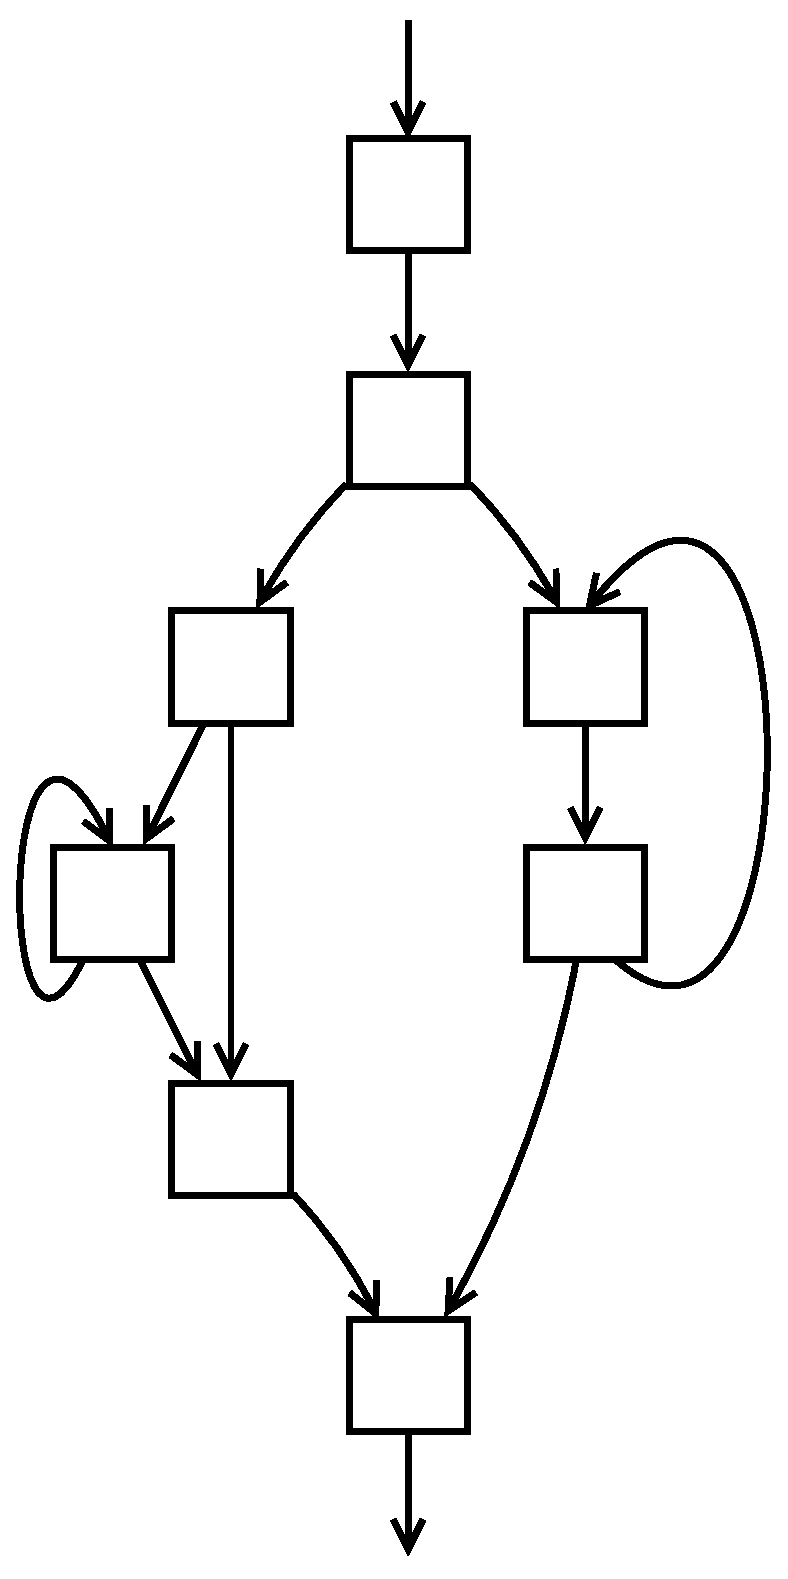
\includegraphics[width=0.15\textwidth]{SimpleRegionCFG.eps}
  %\caption{SCoP CFG}
  %\label{fig:PossibleSCoPCFG}  
%\end{wrapfigure}
A static control part is a region with statically known control flow and memory
accesses. As part of the control flow graph it is restricted to have one entry
edge and one exit edge while loops and conditionals are allowed inside.
To predict all accesses, it is necessary to restrict loop bounds and branch 
conditions to be affine with respect to invariant parameters 
and surrounding iteration variables, but only if they are canonical. 
Because dependency information are crucial for data flow information,
SCoPs are not allowed to contain aliasing instructions at all. 
Furthermore only affine access functions will yield a precise result as 
non affine ones are overestimated (but not forbidden per se).
The last point concerns called function as only side effect free functions
ones are allowed here.
%Figure \ref{fig:PossibleSCoPCFG} shows the CFG of SCoP 

While the code can be transformed to fulfill some of these conditions 
(e.g., the canonical induction variables), the remaining ones are still 
quite restrictive. The desired results, namely the SCoPs, are valuable because
they can be represented within the polyhedral model, thus further analyses and
transformations do not need to deal with the details of the represented code.

Although all regions fulfilling these requirements are
technically SCoPs, we will restrict ourself to those containing at least one loop.

%\begin{table}[htbp] 
  %\centering
  %\caption{Restrictions on SCoPs}
    %\begin{itemize}
      %\item Only nested loops and conditionals
      %\item Only branches with affine conditions
      %\item Only affine accesses based on a constant pointer
      %\item No unsigned iteration variables \footnote{}
      %\item No aliasing instructions
      %\item Only canonical PHI nodes and induction variables
      %\item Instructions may not be used in PHI nodes outside the region\footnotemark[1]
      %\item Only ``readnone'' function calls
      %\item No alloca or cast instructions within the region
      %\item Only affine trip counts for loops
      %\item No PHI nodes in the region exit block
      %\item Only simple regions not containing the entry block of the function
      %%\item \textit{A SCoP should contain at least one loop}
    %\end{itemize}
    %\flushleft{\footnotemark[1] open for further work }
  %\label{tab:SCoPConstraints}
%\end{table}



\subsection{SCoP Detection}
Pollys SCoP detection is the gateway to all further analyses and 
transformations. All regions fulfilling the properties described in the 
last section, or in short, all (valid) SCoPs are detected here. 
The special interest of this part arises from the fact that all 
regions declared as valid SCoPs will be considered for polyhedral 
optimizations. Almost regardless of their content, any region could be given to
Polly if the SCoP detection is properly instrumented. Two important consequences
can be derived and summarized as:
Utilizing the strength of Polly is possible in much more situations as 
intentionally implemented but coupled with responsibility of the outcome.

\subsection{Loop Optimizations}
Polly uses the integer set library (isl) to compute the scheduling and
tiling for a SCoP. Once the polyhedral representation is computed,
an optimized version of the  algorithm proposed by Bondhugula et 
al.\cite{Bondhugula:2008:PAP:1379022.1375595}
will compute a new scheduling and tiling scheme. 
Traditional loop optimizations such as blocking, interchange, splitting,
unrolling or unswitching are implicitly applied during this step. 
%Not only the new scheduling but also the new data dependencies are computed, 
%crucial to exploit parallelism.
%Based on these dependencies parallelism is exploited as explained in the next section. 

%\textit{The loop optimizations offers many possibilities in the context 
%of Sambamba (see \ref{FurtherWorkISL}).}


\subsubsection{Parallel Code Generation}
While cache locality is implicitly improved by rescheduling and tiling 
of the loop nest,  parallel code needs to be generated explicitly afterwards.
Polly is capable of generating
thread level parallelism using OpenMP annotations and data level parallelism 
using SIMD instructions. 
%The former one depends on the OpenMP shared library 
%being present while the later one uses the LLVM built-in vector instruction.
If the former one is desired, the first loop without any loop carried 
dependencies will be rewritten as if there were OpenMP annotations in the first
place. Enabling the later one, namely vector code generation, 
will not only try to vectorize the innermost loop but also the 
scheduling in order to  allow this in more cases.

%\begin{figure}[htbp]
  %\centering
  %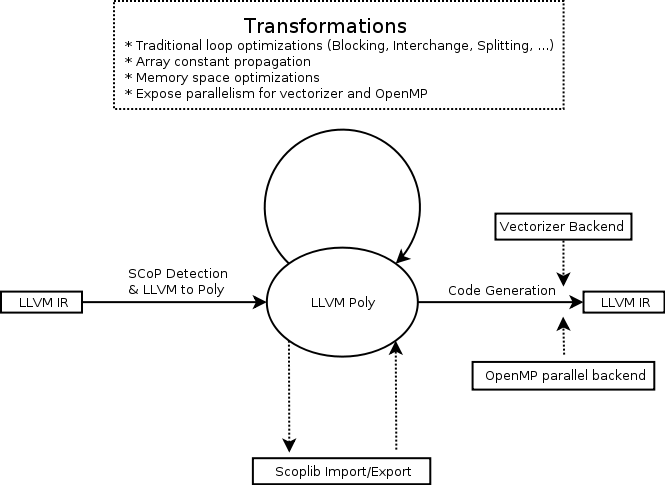
\includegraphics[width=0.9\textwidth]{architecture.png}
  %\caption{Pollys architecture \cite{Polly:Online}}
  %\label{fig:PollyArchitecture}  
%\end{figure}


\subsection*{Further Reading}

\begin{itemize}
  \item Polly - Polyhedral optimization in LLVM \cite{grosser.11.impact}  
  \item Enabling Polyhedral Optimizations in LLVM \cite{grosser:thesis}
  %\item A Framework for Automatic OpenMP Code Generation \cite{raghesh2011framework}
  \item Base algorithm of isl \cite{Bondhugula:2008:PAP:1379022.1375595}
  \item \url{http://polly.llvm.org} \nocite{Polly:Online}
  \item \url{http://www.kotnet.org/~skimo/isl/} \nocite{ISL:Online}
\end{itemize}





\clearpage
%\phantomsection
%\addtocounter{section}{1}
%\setcounter{subsection}{1}
\section[Sambamba - A Framework For Adaptive Program Optimization]{Sambamba \\ A Framework For Adaptive Program Optimization}
%\addcontentsline{toc}{section}{2.4 ~ Sambamba - A Framework For Adaptive Program Optimization} 
%The Sambamba project is build on top of the LLVM compiler infrastructure and 
%aims at adaptive and speculative runtime optimizations.
%Dynamic information about arguments or the global state may allow optimization
%which could not be applied at compile 
%\begin{wrapfigure}[]{r}{0.3\textwidth}
  %\centering
  %%\vspace*{-5mm}
  %\includegraphics[width=0.3\textwidth]{SambambaConcept.eps}
  %\caption{Sambamba in a nutshell}
  %\label{fig:SambambaConcept}  
%\end{wrapfigure}
%time or did not seem interesting back then. It is easily extendible with 
%compile time and a runtime parts. While each one is conceptually 
%independent, the compile time parts may store information which can be accessed
%at runtime to reduce the overhead, even if expensive analysis results are needed. 
%Another fundamental pillar of the framework is the multi versioning system which
%allows for different, specialized function versions.
%[TODO FILL THIS PAGE ]
%%[TODO should VMAD be mentioned here]
%%A similar approach has
%%been published by Jimborean et al.\cite{JIMBOREAN-2012-664345}, in fact th
%%In both cases a dispatcher is used to choose one of the available 
%%implementations each time the function is called. 
%%In this manner exclusive optimizations can be applied on the same function and
%%according to the input a version can be dispatched. Runtime profiling also 
%%reveals opportunities to speculatively transform the program and obtain more
%%specialized versions. A main difference between Sambamba and the work of 
%%Jimborean is probably how these function versions are constructed. Sambamba does
%%not rely on source code annotations but allows all modules to find and extract
%%the versions fully automatic. 
%A high level view on the Sambamba concept is given
%by figure \ref{fig:SambambaConcept} before some of the  built-in utilities 
%and modules, used during this work, are explained. 
\begin{wrapfigure}{r}{0.3\textwidth}
  \vspace*{-4mm}
  \centering
  \includegraphics[width=0.3\textwidth]{SambambaConcept.eps}
  \caption{Different stages in the Sambamba framework}
  \label{fig:SambambaConcept}
  \vspace{-4mm}
\end{wrapfigure}
As an extension to LLVM the Sambamba compiler framework is designed to
allow runtime analyses and (speculative) optimization.
Furthermore these optimization can create and refine runtime profiles which
are used to recalibrate and specialize the (speculative) execution. Method 
versioning allows conservative and speculative 
versions of a method to be stored and switched during runtime. 
%But both can profit from specialization at runtime. 
%especially after conflicting speculation.
%Based on the LLVM suite, Sambamba uses the shipped JIT compiler 
%and a software transactional memory system to secure
%speculative execution. 
Written in a completely modular way, Sambamba extensions consist 
of a static part (compile time) and a dynamic one (runtime). 
Both extension parts can use Sambamba to store information,
collected at the corresponding time, accessible for the dynamic part at 
runtime.
%In the context of speculation and profiling, Sambamba can be used to store
%several version of a method which can be generated by one of the two parts.
Profiling combined with the method versioning system allows runtime interactions
to explore more parallelism or minimize the overhead in case of misspeculation. 

\paragraph{Stages in the Sambamba framework\\} ~\\
As illustrated in Figure \ref{fig:SambambaConcept} we can differentiate five stages
embedded in the Sambamba framework.

{\begin{list}{}
    {\setlength{\leftmargin}{-0mm}}
  \item[]
\begin{enumerate}
  \item[\textbf{[A]}] Execute static whole-program \textbf{analyses}  
  with the possibility to save their results.
\item[\textbf{[P]}] Speculatively \textbf{parallelize} parts of the program
  based on the results of \textbf{[A]} and \textbf{[S]}.
\item[\textbf{[X]}] Detect and recover from conflicts by speculative
  \textbf{execution} using a software transactional memory system.
\item[\textbf{[C]}] Use the profiles and misspeculation information gained 
  during the execution to \textbf{calibrate} future optimization steps.
\item[\textbf{[S]}] Generate \textbf{specialized} variants of a function, 
 one for each special input profile detect by \textbf{[C]}. 
\end{enumerate}
\end{list}
}




\clearpage
\subsection{Sambambas Parallelizer}
\begin{wrapfigure}[]{l}{0.40\textwidth}
  \centering
  %\vspace*{-10mm}
  \includegraphics[width=0.38\textwidth]{TransactionQueue.eps}
  \caption{Symboliced transaction queue with three worker threads}
  \label{fig:TransactionQueue}  
\end{wrapfigure}
The Sambamba parallelizer will become the main interface for any kind of 
parallelization in the framework. At the moment it is in need of parallel control
flow graphs to explicitly state section which should be executed in parallel, but
in the future an automatic loop parallelization component will be implemented too. 
The runtime part of the parallelizer instantiates as many worker threads as 
there are cores on the executing machine. Each worker thread will later on execute 
one transaction at a time. In contrast to the OpenMP approach
no external libraries are needed to exploit parallelism. \\


\subsection{Parallel Control Flow Graphs}
\begin{wrapfigure}[]{r}{0.35\textwidth}
  \centering
  \vspace*{-2mm}
  \begin{minipage}[c][0.37\width]{\textwidth}
  \includegraphics[width=0.33\textwidth]{ParallelSectionEx.eps}
  \end{minipage}
  \caption{A parallel section with three transactions}
  \vspace*{-3mm}
  \label{fig:ParallelSectionEx}  
\end{wrapfigure}
A parallel control flow graph (ParCFG) is a data structure used by the
parallelizer to express parallel sections within an ordinary CFG. 
Each parallel sections consist of an entry block called \texttt{piStart} and
an exit block called \texttt{piEnd}. The \texttt{piStart} is terminated by a 
symbolic switch statement which may have an arbitrary number of successors. 
Every successor denotes a, so called, transaction which ends in the 
\texttt{piEnd} block after some arbitrary computation. 
To put it in another way, parallel sections correspond to
fork-join parallelism where the \texttt{piStart} blocks forks transactions 
which are synchronized at the \texttt{piEnd} block. In the case of Sambamba this
synchronization is done by a software transaction memory as described in the 
next section.

Figure \ref{fig:ParallelSectionEx} shows such a parallel section with three 
highlighted transactions. At runtime they will be executed concurrently, each 
by one worker thread at a time.
\\

\subsection{Software Transactional Memory}
A software transactional memories (STM) is a conflict management system used to detect
memory conflicts in speculatively parallelized programs and closely related to
the transaction system in databases. When in use the STM logs
all accesses to the memory from the beginning of a transaction up to the 
synchronization. If, during this time, a memory address has been written and 
read by different threads, the reading ones might have worked with
corrupted data, thus all resulting computations might be wrong. In such a case
the STM will force the threads to recompute theirs results. There are different
implementations which will, for example, allow at least one thread finish its
computation before all other might have to recompute theirs. Such implementations 
will always preserve the liveness of a system as there is progress, even though
the required time might be quadratic in the number of threads.

As the described implementation only preserves liveness but no ordering between
the different computations, you might want to use, so called, commit orders. 
A commit is the final synchronization step of a thread in an STM environment and
a commit order will enforce the threads to synchronize, thus store their result
permanently, in the exact same order as they have been created. Just like the 
unordered version this one guarantees liveness.

Another possible extension for an STM system is a wait construct which is build
on top of the commit order. Such a wait will cause the thread to pause until 
all other threads, in front in the commit order, have passed a corresponding 
barrier, intentionally placed only a few instructions behind the wait. The 
enclosed instructions would form a mutual exclusive area which can only be 
entered by one thread at a time. 


The current STM implementation in the Sambamba framework does neither provide a 
commit order nor the wait construct, but this will change in the future.

\subsection*{Further Reading}
\begin{itemize}
  \item Sambamba: A Runtime System for Online Adaptive Parallelization \cite{DBLP:conf/cc/StreitHZH12}  
  \item \url{http://www.sambamba.org} \nocite{StreitHZH12:Online}
\end{itemize}



